\chapter{Hardware Detail Design}
\label{chap:5}

This chapter gives a detailed discussion on the hardware design and
configuration of this system. 

\section{Relay Switch Circuit}
\label{sec:detail-switch}

As explained in Section \ref{sec:relay-switch} in page \pageref{sec:relay-switch}, a relay
switch (the Mantech NT72C 12V DC relay [\cite{manual:relay-specs}]), in conjunction with a 2N2222
Bipolar Junction Transistor (BJT) [\cite{maunual:transistor-datasheet}], is used
by the Raspberry Pi to switch the motor on and off. See Figure
\ref{fig:relay-switch} for the circuit diagram.

\begin{figure}
\centering
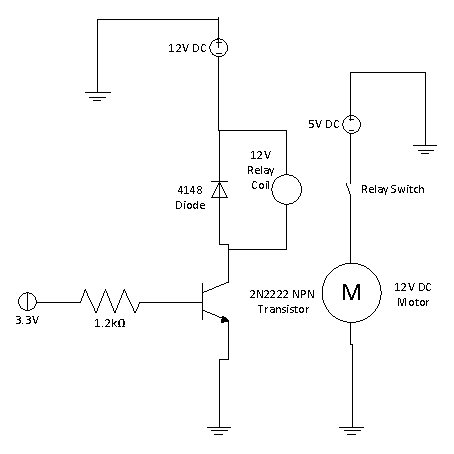
\includegraphics[scale=0.7]{relay_switch.eps}
\caption{12V relay transistor switch.}
\label{fig:relay-switch}
\end{figure}

The relevant  parameters for these components are [\cite{manual:relay-specs},
\cite{maunual:transistor-datasheet}]:

\[ P_{r} = 0.36W\]
\[ V_{r} = 12V\]
\[ \beta \approx 10\]
\[ V_{p} = 3.3V\]

From the relays power dissipation and voltage, its current draw is found by

\[
I_{r} = \frac{P_{r}}{V_{r}}
\]

which gives a current draw of

\[
I_{r} = 0.03A
\]

Taking the BJT's current amplification as roughly 10, the current draw from the Pi to the
base of the BJT is given by

\[
I_{b} = \frac{I_{r}}{\beta} = \frac{I_{c}}{\beta}
\]

This gives a current draw of

\[
I_{b} = 0.003A = 3mA
\]

The maximum current draw from the GPIO pins is 16mA [\cite{website:gpio-specs}], though this is
not recommended as the Pi does not have any current limiting or over-current protection.
Therefore, a current draw of 3 mA is completely safe.

To limit the current draw from the Pi, a base resistor must be added between the Pi's GPIO pin
and the BJT's base. With a current draw of $3mA$ and a voltage of $3.3V$, the resistor size is
found by Ohm's law as follows

\[
R_{b} = \frac{V_{p}}{I_{p}}
\]

which gives

\[
R_{b} = 1.1k\Omega
\]

Compensating for tolerances by adding 10\%, the resistor size is set to

\[R_{b} = 1.2k\Omega\]

which draws a current of 

\[I_{b} = 2.75 mA \]

which is still within the acceptable range.

\section{NFC Chip}

The Near Field Communication (NFC) chip used, is the Adafruit NFC shield for an
Arduino Uno microcontroller [\cite{website:adafruit-nfc}]. See Section
\ref{sec:nfc-controller} on page \pageref{sec:nfc-controller} for more details on the controller.

The shield was designed and built to be used by an Arduino Uno microcontroller.
Therefore, some modification to the chips connections had to be made before it
would be able to communicate with the Pi.

By default, the chip was made to communicate with an Arduino with the Inter
Integrated Circuit ($I^2C$) communication protocol. However, the component
manufacturers have added connection pads to the chip that, when soldered, allows
the chip to communicate via Serial Peripheral Interface (SPI) or Transistor
Transistor Login (TTL). 

The libnfc library is currently only configured to allow communication via an
Universal Asynchronous Receiver Transmitter (UART). Therefore if the chip was
modified to communicate via its TTL interface, which is compatible with a UART. 

To do this, the `SEL1' pads were soldered closed (see Figure
\ref{fig:nfc-chip-solder}). With this done, the chip can serially communicate
with the Raspberry Pi's UART interface.

\begin{figure}
 \centering 
 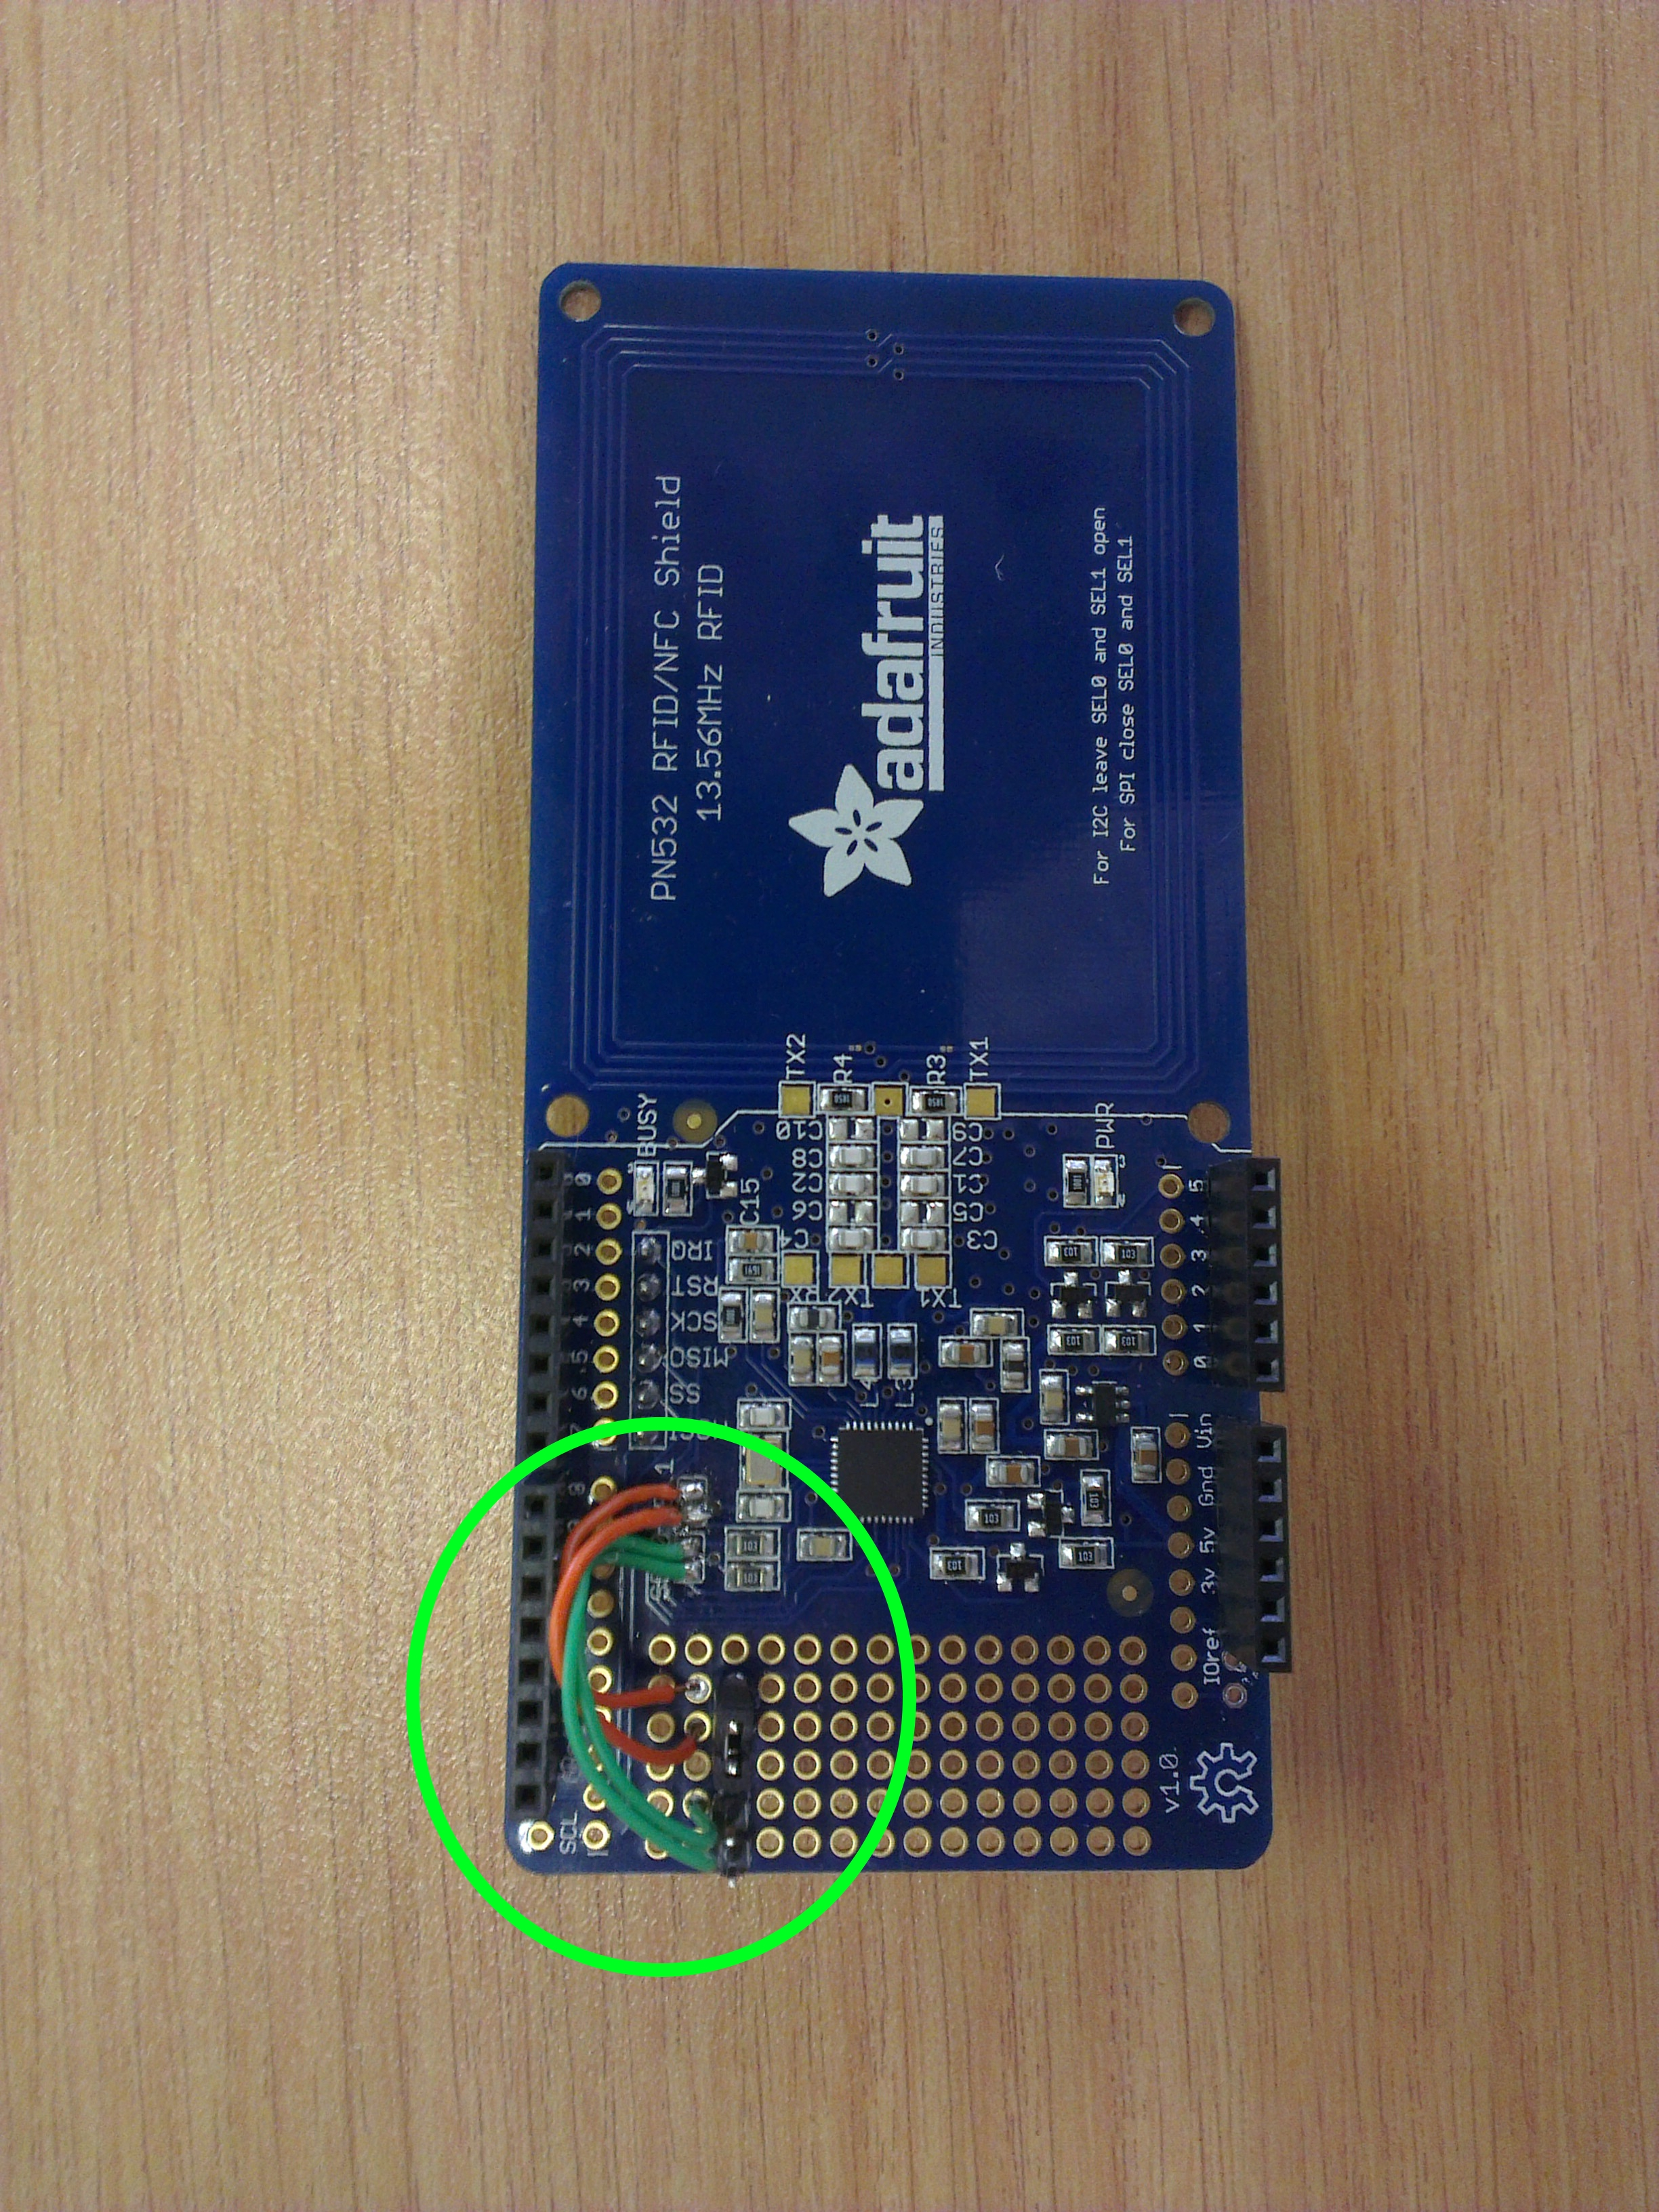
\includegraphics[clip=true, trim = 0 250 0 270,
 scale=0.7]{soldeer_pic}
 \caption{The location of the SEL1 pads (highlighted in green).}
 \label{fig:nfc-chip-solder}
\end{figure}

The connections between the Pi and the NFC controller are as follows: 

\begin{table}
\centering
 \caption{Connections between the Raspberry Pi and the NFC Controller chip.}
 \begin{tabular}{|l|l|l|}
  \hline
  \textbf{NCF Controller Pin} & \textbf{Raspberry Pi Pin}\\\hline\hline
  5V pin & 5V (pin 4) \\\hline
  Ground pin & Ground pin (pin 6) \\\hline
  SS & UART0 TXD (pin 8) \\\hline
  MOSI & UART0 RXD (pin 10) \\\hline
 \end{tabular}
\end{table}

\section{libnfc Setup on the Raspberry Pi}

Before libnfc could be built and configured, the communication between the NFC
controller and the Pi needed to be finalised. To do this, the Pi's UART needed
to be freed up. By default, the Raspberry Pi uses its UART to serially write out
its booting information. Therefore, to allow the Raspberry Pi to communicate
with the NFC controller via its UART0 interface, it was necessary to modify
some of its configuration files. To do this, the Adafruit tutorial was followed
[\cite{website:adafruit-tutorial}].

To do this, the file `/boot/cmdline.txt' and `/etc/inittab' had to be edited to
contain the following lines of code:\\\\

\textbf{cmdline.txt}
\begin{verbatim}
dwc_otg.lpm_enable=0 console=tty1
\end{verbatim}

\textbf{inittab}
\begin{verbatim}
#Spawn a getty on Raspberry Pi serial line
#T0:23:respawn:/sbin/getty -L ttyAMA0 115200 vt100
\end{verbatim}

After this has been done, the libnfc package could be configured and installed
and configured to work with the Pi's UART interface.

Thereafter, the Pi is ready to receive NFC messages from the
NFC shield.

\section{Vending Machine Unit}

A small vending machine unit was constructed for demonstration purposes. It is
designed to house all the vending machine components, i.e. the two DC motors,
the two coils, the Raspberry Pi central controller, the NFC shield and the
webcam.

Four 10mm vent holes were added at the sides to improve air circulation
and to provide external wire access, while a larger 60mm vent hole was also
added to allow for an external 60mm desktop computer fan to be added. 

The unit is made from 1.6mm thick mild steel and the components were cut and
bent by Fabrinox, Paarl and welded together by the Electric and Electronic
Engineering Department of Stellenbosch University's workshop.

See Figure \ref{fig:vm-actual} for a picture of the
complete vending machine unit with the two DC motor
inserted. See Appendix \ref{app:vm-tekeninge} for detailed
design drawings of the vending machine unit.

\begin{figure}
 \centering 
 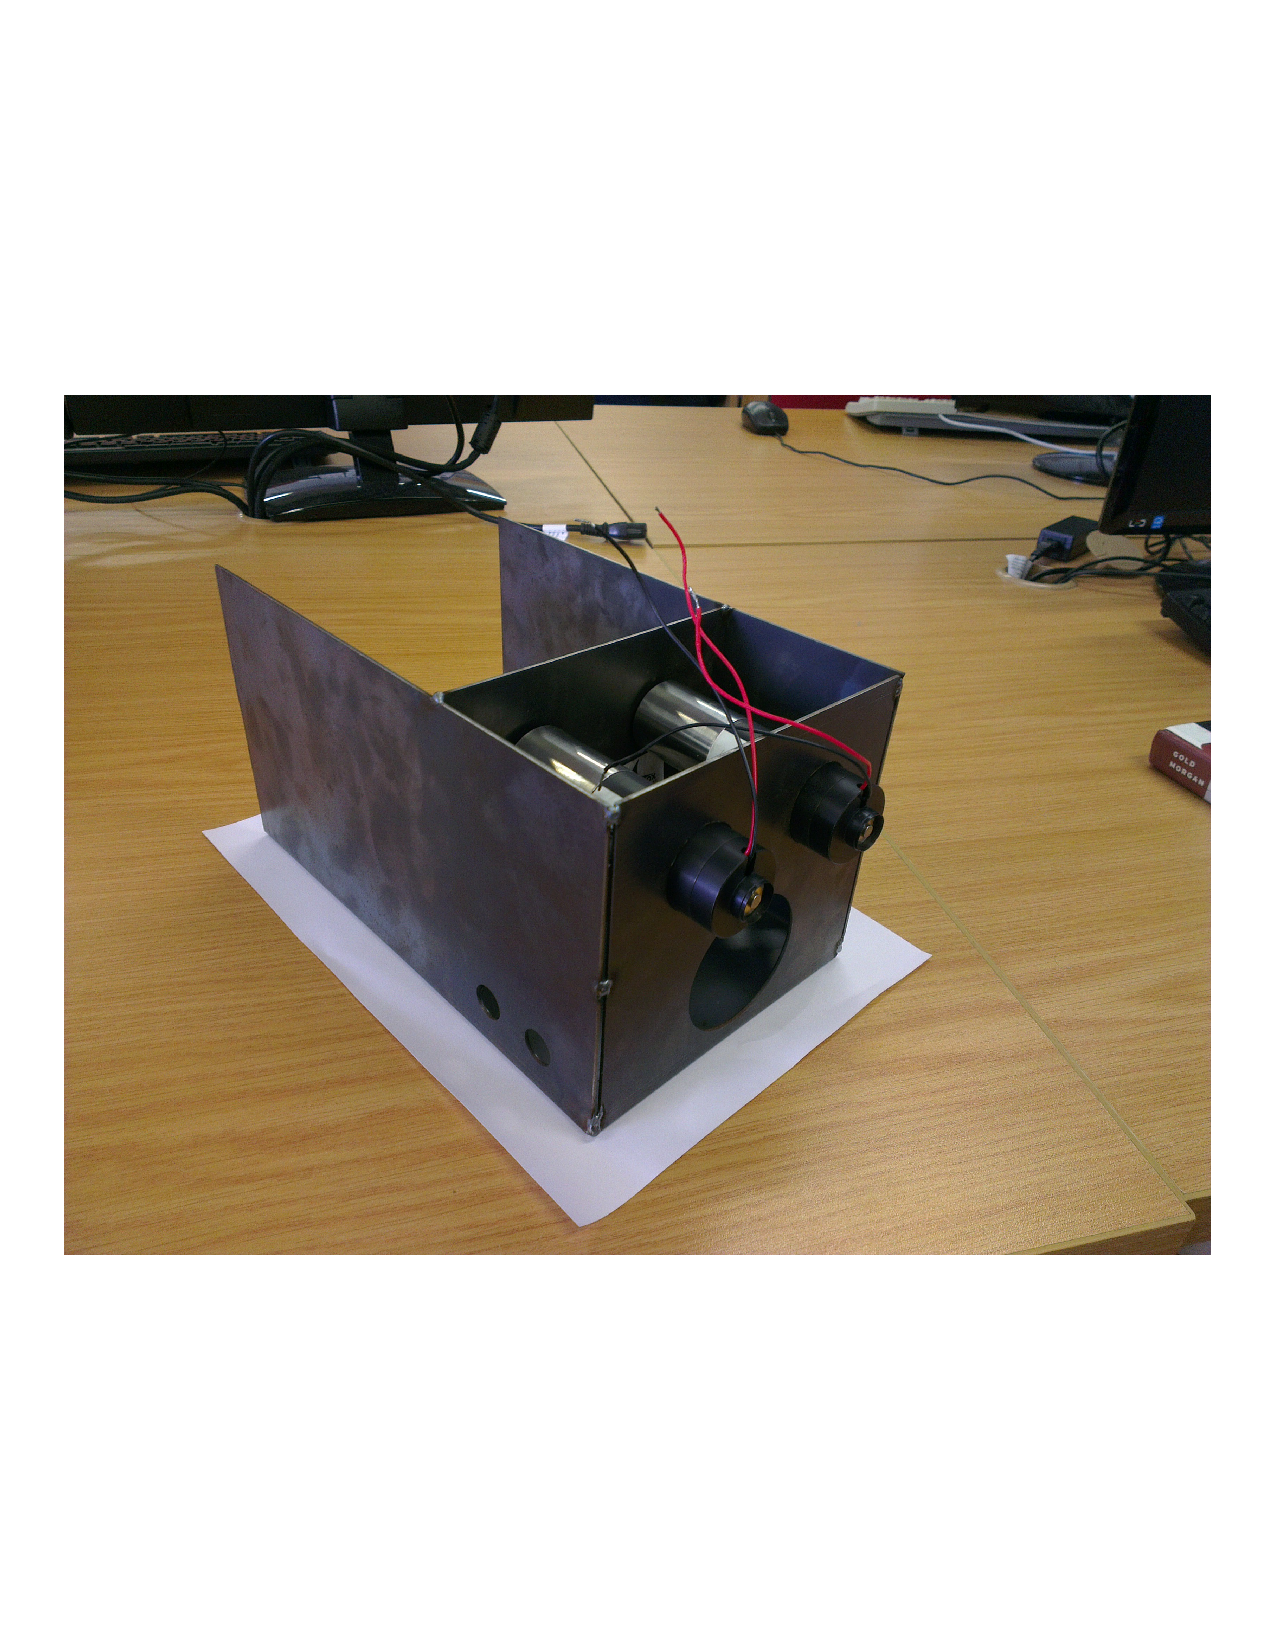
\includegraphics[clip=true, trim = 80 150 150 200,
 scale=0.7]{complete_vm}
 \caption{The complete vending machine unit.}
 \label{fig:vm-actual}
\end{figure}

\section{Webcam}

As discussed in Section \ref{sec:webcam}, a Sony PS2 Eye Toy  webcam was
attached to the Raspberry Pi. This allows the vending machine to scan a live
video feed for a QR Code. Its already compatible with the Raspberry Pi and
therefore requires minimal configuration to begin working.

However, the camera needs to be plugged into a Universal Serial Bus (USB) port
on the Pi itself and not into a USB hub. This is done in order to prevent the
hardware timing issues that are introduced to the system when a USB hub is used. 

\section{Motor and Coil}

MOET NOG GEDOEN WORD.




